% Rotación de un vector en 2D (libro fig. 1.2)
\documentclass[border=4pt]{standalone}
\usepackage{tikz}
\usetikzlibrary{arrows.meta}
\begin{document}
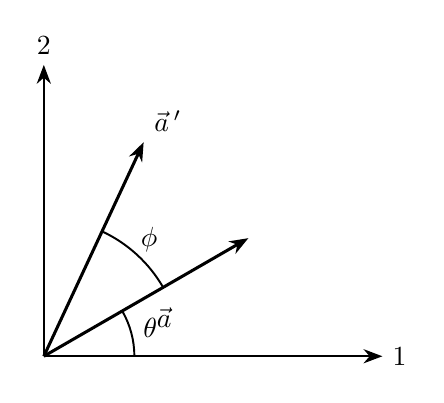
\begin{tikzpicture}[>={Stealth[length=2.4mm]}, line width=0.7pt]
  \draw[->] (0,0)--(4.3,0) node[right]{$1$};
  \draw[->] (0,0)--(0,3.7) node[above]{$2$};
  \coordinate (O) at (0,0);
  \draw[->, line width=1.1pt] (O)--(30:3) node[midway,below right]{$\vec a$};
  \draw[->, line width=1.1pt] (O)--(65:3) node[above right]{$\vec a\,'$};
  \draw (1.15,0) arc (0:30:1.15); \node at (15:1.4){$\theta$};
  \draw (30:1.75) arc (30:65:1.75); \node at (48:2.0){$\phi$};
\end{tikzpicture}
\end{document}
